\section{PSYCHE with a variable number of saltires}
\label{sec:pureshift__nsaltire}

\begin{figure}[htb]
    \centering
    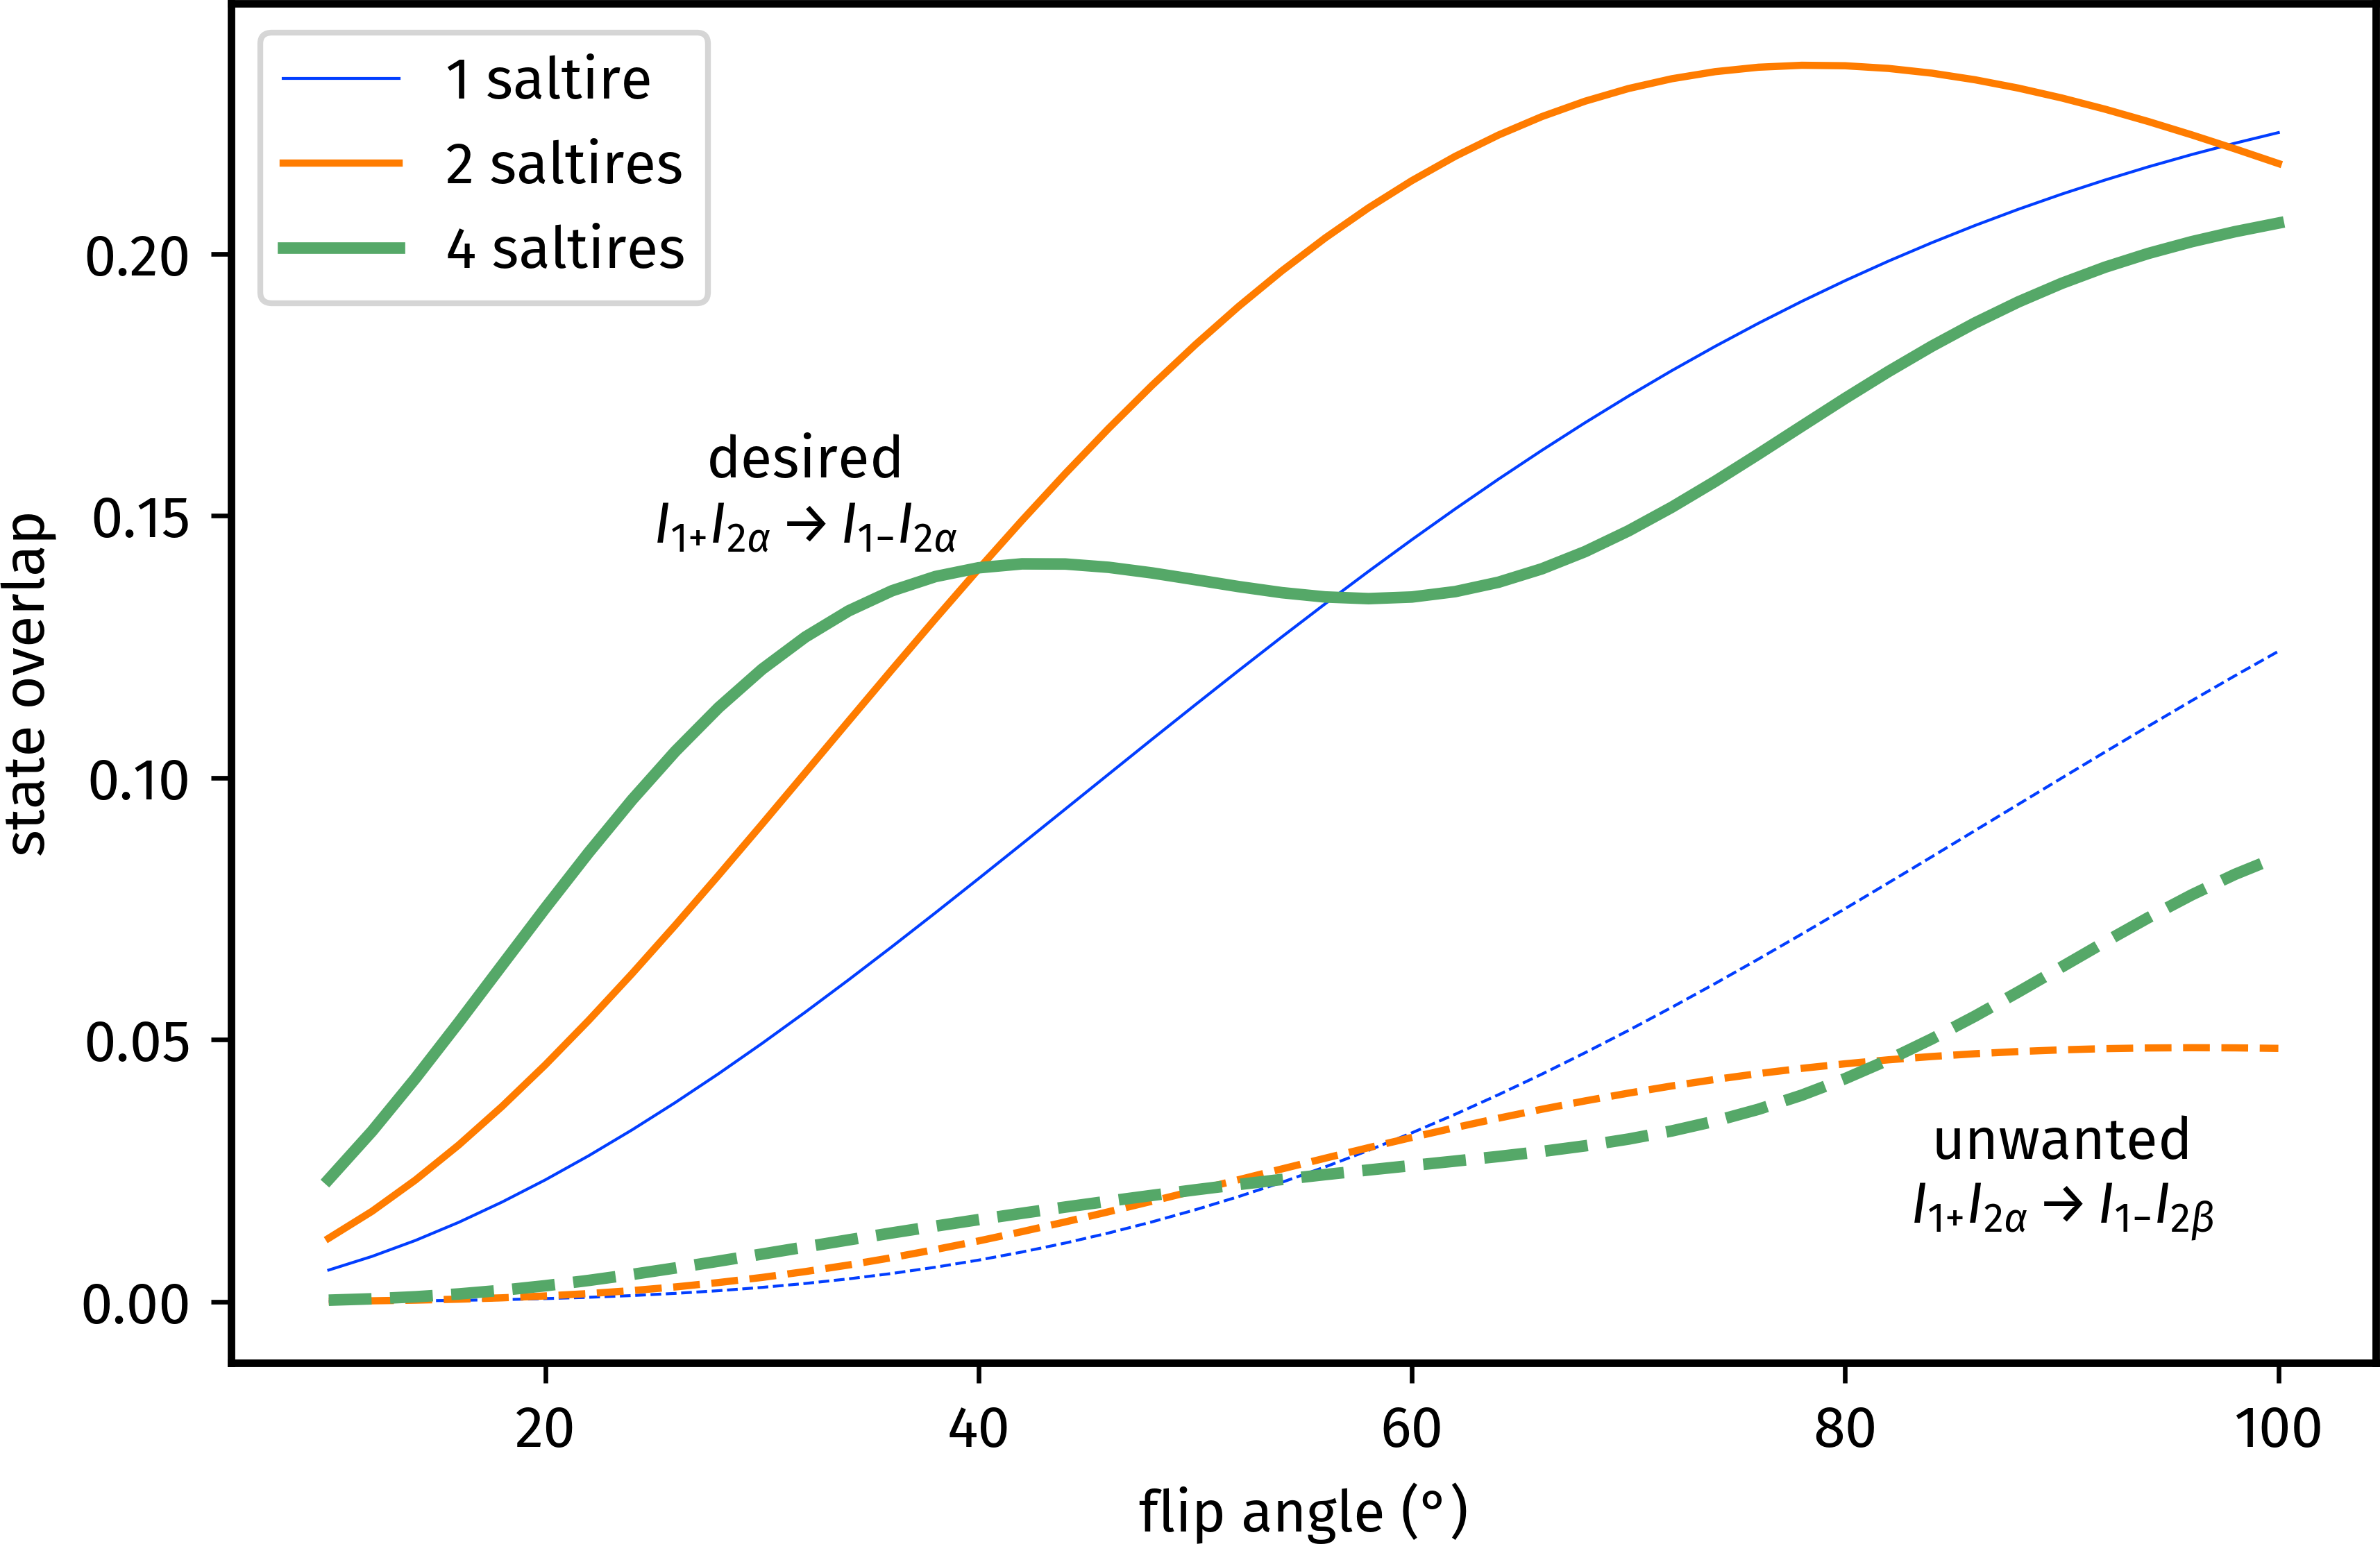
\includegraphics[]{pureshift/fa_dependence_124.png}
    \caption[Signal and artefact intensity with 1-, 2-, and 4-saltire PSYCHE]{Simulated signal and artefact intensity for various PSYCHE-style PSEs as a function of the flip angle used.
    Calculations were performed on a two-spin system with a coupling of \SI{7}{\Hz}, and an offset difference of \SI{1.5}{\kHz}.
    The total PSE duration was \SI{30}{\ms} (so, for example, in the four-saltire PSYCHE, each saltire was \SI{7.5}{\ms}).
    Solid lines indicate the coefficients for the desired $I_{1+}I_{2\alpha} \to I_{1-}I_{2\alpha}$ pathway which contributes to the pure shift signal; dashed lines the coefficients for the undesired $I_{1+}I_{2\alpha} \to I_{1-}I_{2\beta}$ pathway, which gives rise to recoupling artefacts.
}
    \label{fig:fa_dependence_124}
\end{figure}

The first attempted method was to change the number of saltire pulses used in the waveform.
As described above, PSYCHE relies on spatiotemporal averaging to suppress unwanted artefacts: this crucially relies on the fact that the pulse(s) used in the PSE are symmetric.
This can be accomplished with two opposing chirps, or two saltires, both of which are symmetric.
However, a \textit{single} saltire is also symmetric in itself: it is not hard to show that the analysis given in \cref{subsec:pureshift__psyche_analysis} is still valid for a single saltire.
Likewise, the use of four saltires would also be valid.

Theoretical simulations show that the overall profile of signal and artefact versus flip angle (unsurprisingly) varies with the number of saltires: in particular, using more saltires with a smaller flip angle generally accomplishes a similar effect (\cref{fig:fa_dependence_124}).
This may be qualitatively rationalised as more saltires providing more possible CTPs which generate the desired signal (the same idea is generally invoked when discussing the difference between unidirectional chirps and saltires\autocite{Foroozandeh2018CEJ}).
However, regardless of the number of saltires, the fundamental strategy of adjusting the flip angle to control the signal-to-artefact ratio remains valid, which naturally raises the question of whether specific pulse parameters can be chosen in order to obtain the best decoupling quality.

\begin{figure}[htb]
    \centering
    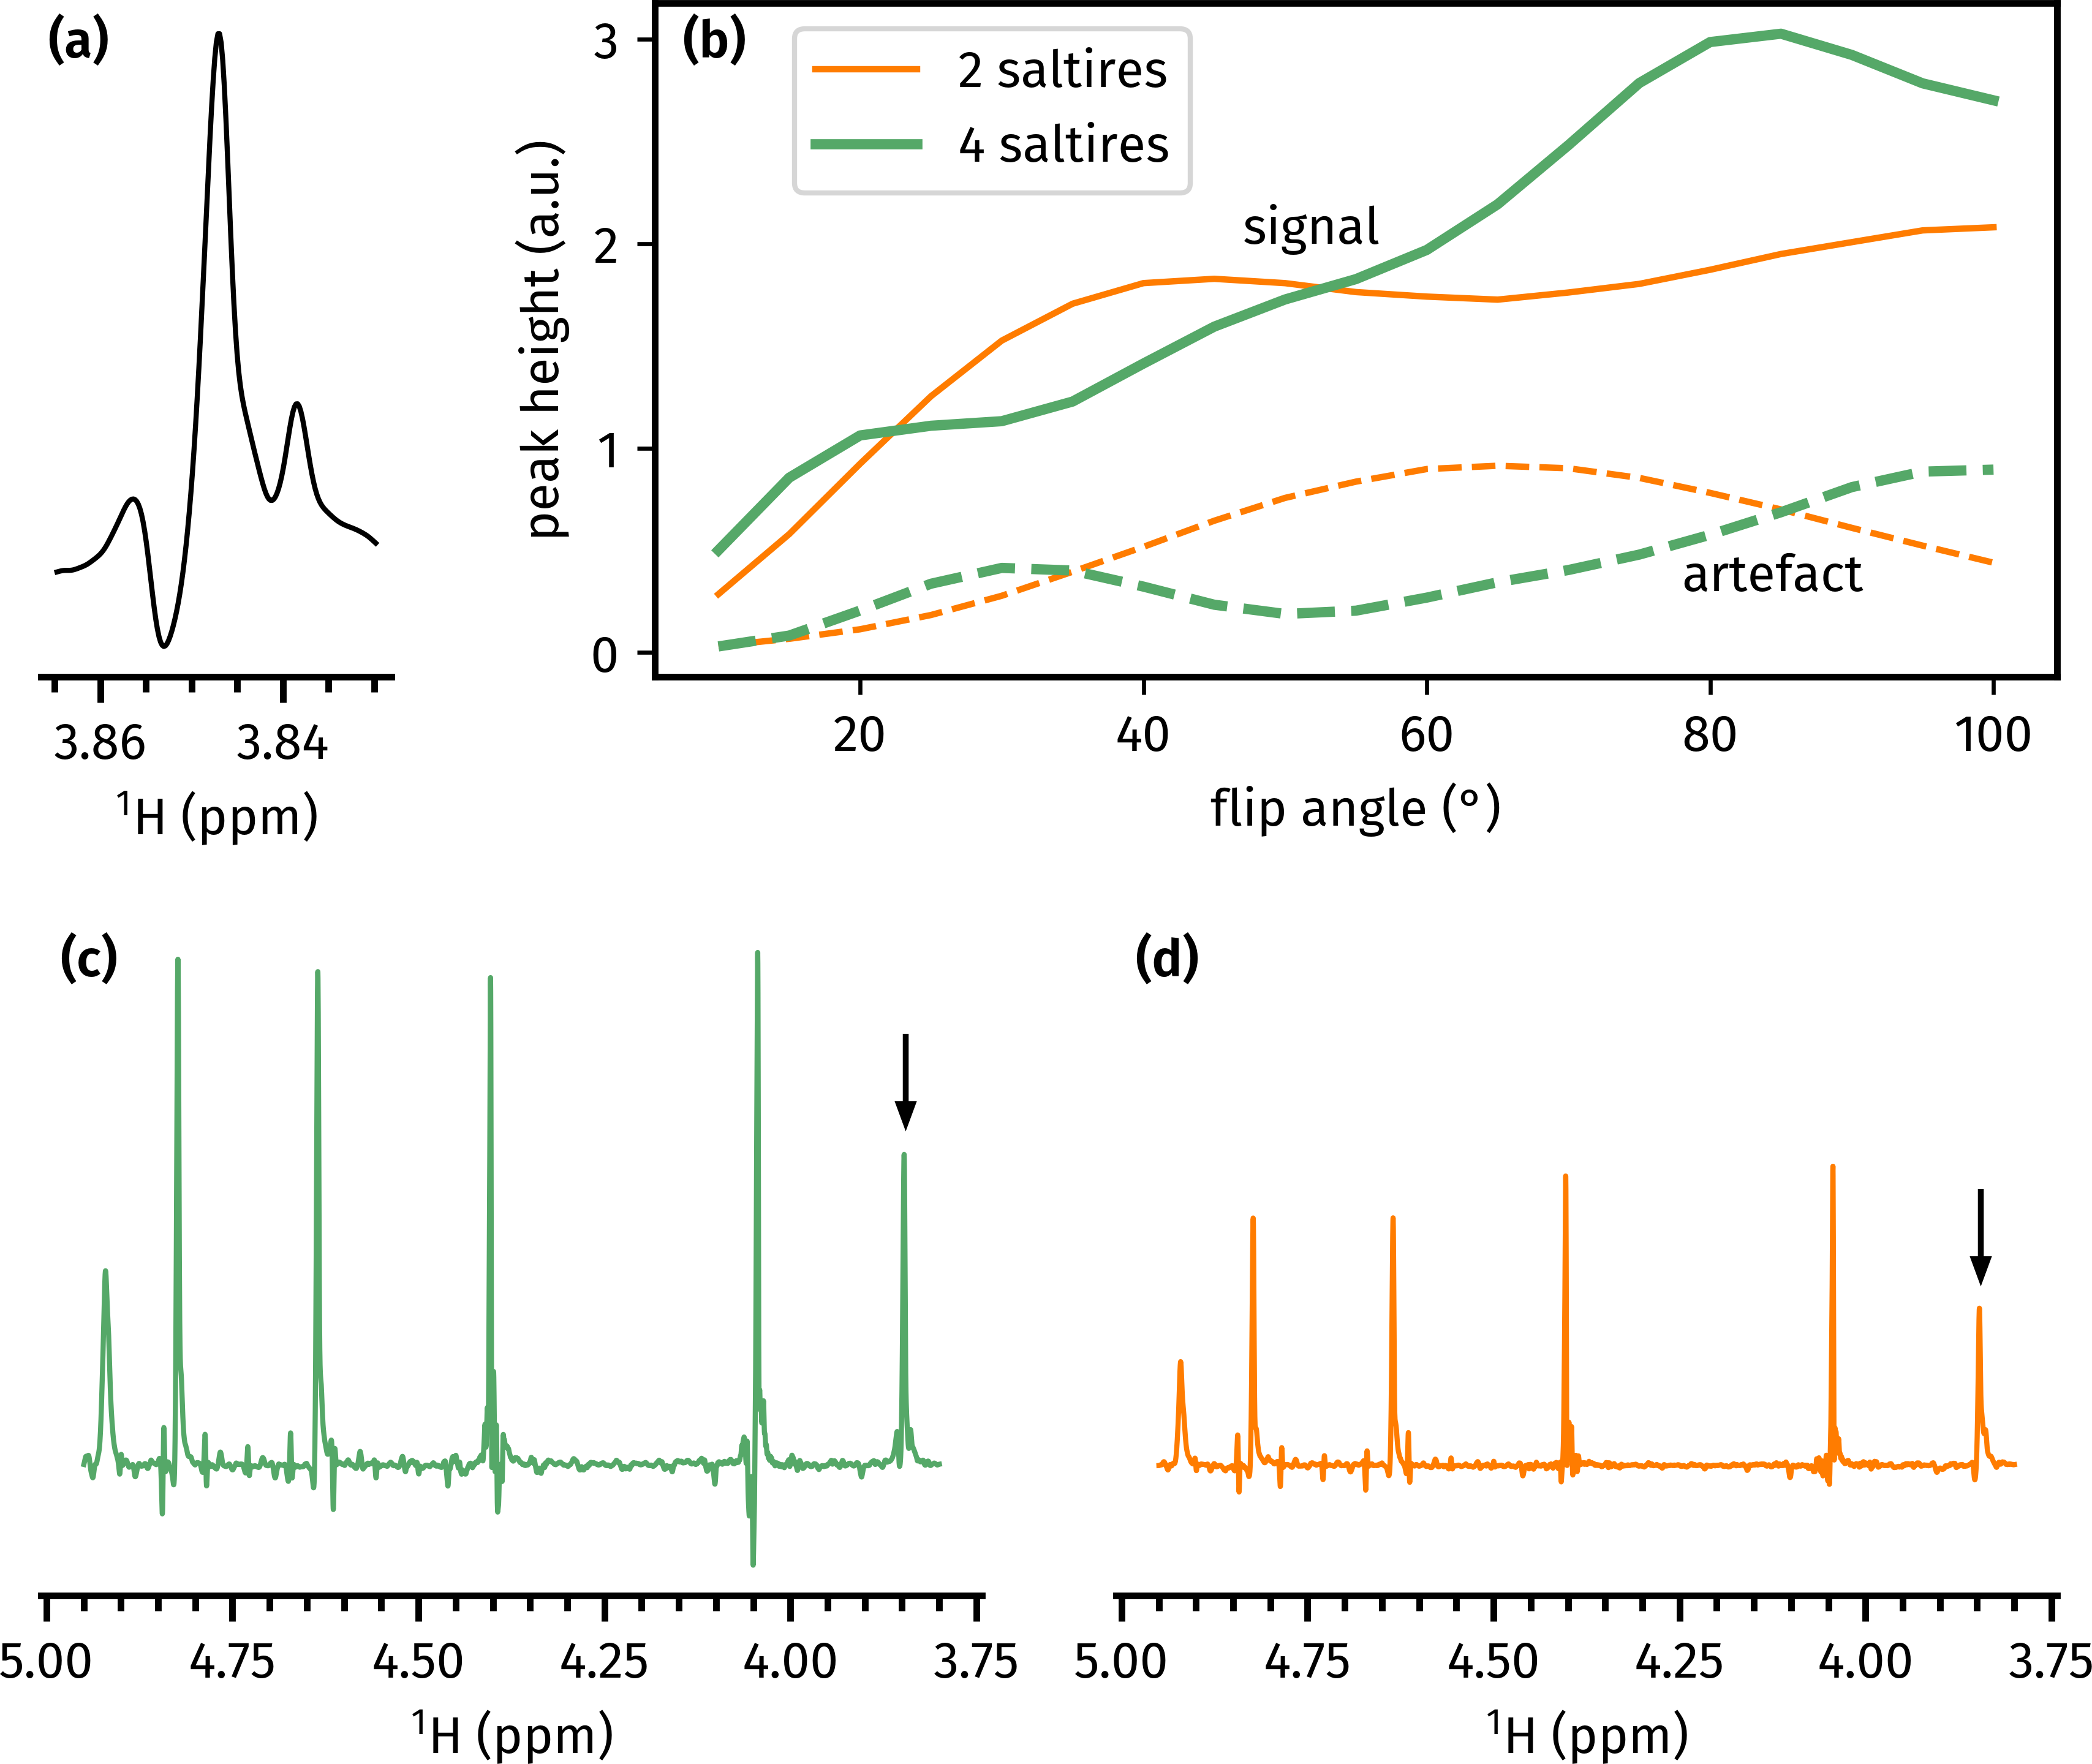
\includegraphics[]{pureshift/quadruple_saltire_30ms.png}
    {\phantomsubcaption\label{fig:quadruple_saltire_30ms_spec}}
    {\phantomsubcaption\label{fig:quadruple_saltire_30ms_plot}}
    {\phantomsubcaption\label{fig:quadruple_saltire_30ms_maybebetter}}
    {\phantomsubcaption\label{fig:quadruple_saltire_30ms_reference}}
    \caption[Comparison of 30 ms double saltire and 30 ms quadruple saltire]{
        \textbf{(\subref{fig:quadruple_saltire_30ms_spec})} The peak in the pure shift spectrum of andrographolide used for calculation of signal and artefact intensity.
        The recoupling artefacts flanking the main peak are clearly visible.
        \textbf{(\subref{fig:quadruple_saltire_30ms_plot})} Peak heights of the desired signal (the central peak) and artefacts (the mean of the two flanking peaks), as a function of flip angle.
        \textbf{(\subref{fig:quadruple_saltire_30ms_maybebetter})} Quadruple-saltire PSYCHE with $\beta = 55^\circ$.
        \textbf{(\subref{fig:quadruple_saltire_30ms_reference})} The reference spectrum, a double-saltire PSYCHE with $\beta = 20^\circ$.
        The peak at \SI{3.85}{ppm} used for the sensitivity and purity analysis is labelled with an arrow.
        \datacode{7A-201016}
    }
    \label{fig:quadruple_saltire_30ms}
\end{figure}

We first consider the quadruple-saltire PSYCHE.
In the first instance, we set the total duration of the PSE to \SI{30}{\ms}: this implies that each saltire is \SI{7.5}{\ms} long.
For this experiment, the sensitivity was defined as the maximum height of the main peak in \cref{fig:quadruple_saltire_30ms_spec}, and the artefact as the mean of the maximum heights of the two artefacts surrounding it.
The plot in \cref{fig:quadruple_saltire_30ms_plot} shows how these quantities vary as a function of the flip angle.
Interestingly, for the artefacts, the profile observed is similar to that in the simulations: the double-saltire version performs better at low and very high flip angles, but in the middle there is a region where the quadruple-saltire version has lower artefact intensity.
The signal intensities for both the double- and quadruple-saltire versions, however, seem to plateau off rather more quickly than the simulations suggest.

To highlight one particular data point, \cref{fig:quadruple_saltire_30ms_plot} suggests that the quadruple-saltire experiment with $\beta \approx 55^\circ$ has a similar artefact level to the double-saltire experiment with $\beta \approx 20^\circ$, but with substantially greater signal intensity.
Insets from these two spectra are respectively shown in \cref{fig:quadruple_saltire_30ms_maybebetter,fig:quadruple_saltire_30ms_reference}.
In fact, this conclusion seems to be true for the peak in question, which is at the right edge of the spectral insets shown here.
Overall, the quadruple-saltire \ang{55} experiment does have better sensitivity than the double-saltire \ang{20} experiment.
However, the artefact intensity is not always suppressed as nicely as it is in the chosen reference peak: for example, the peak at \SI{4.05}{ppm} is significantly less clean in the quadruple-saltire experiment.
Any apparent advantage over the double-saltire experiment is therefore not very clear---at least from this data alone.%
\footnote{In fact, I also performed some preliminary experiments where the four-saltire PSE was lengthened to \SI{60}{\ms}. The artefact behaviour in these spectra were better than in their \SI{30}{\ms} counterparts, which is to be expected since a longer PSE leads to better spatiotemporal averaging. However, I unfortunately did not compare these against a \SI{60}{\ms} double-saltire experiment, so these results are not included in this thesis. (It would be rather unfair to compare them against the \SI{30}{\ms} double-saltire.)}

Moving on to the single-saltire case, in addition to searching for a better signal and artefact profile, another possible motivation would be that the duration of the PSE can be decreased.
This would minimise losses due to relaxation and diffusion during the PSE, which were not taken into account in \cref{fig:fa_dependence_124} (and the simulations there did not vary $\taup$ anyway).
A single-saltire PSYCHE experiment was thus recorded with various combinations of flip angle ($\beta/^\circ \in \{15, 20, 25, 28, 30\}$) and pulse duration ($\taup/\text{ms} \in \{15, 25, 30, 35, 45, 55\}$).
In a similar way to the quadruple-saltire study, the sensitivity here was defined as the maximum height of the main peak in \cref{fig:single_saltire_results_spec}, and the artefact as the mean of the heights of the two artefacts surrounding it.
(However, note that the compound used was different.)
The purity, or signal-to-artefact ratio, is simply the former divided by the latter.%
\footnote{As an alternative, the Bruker \texttt{sinocal} AU programme was also used to measure the sensitivity of the spectrum; it yielded extremely similar results, so is not shown here. I found the \texttt{sinocal} routine to be rather unreproducible as the exact value calculated depends on random noise.}

\begin{figure}[htbp]
    \centering
    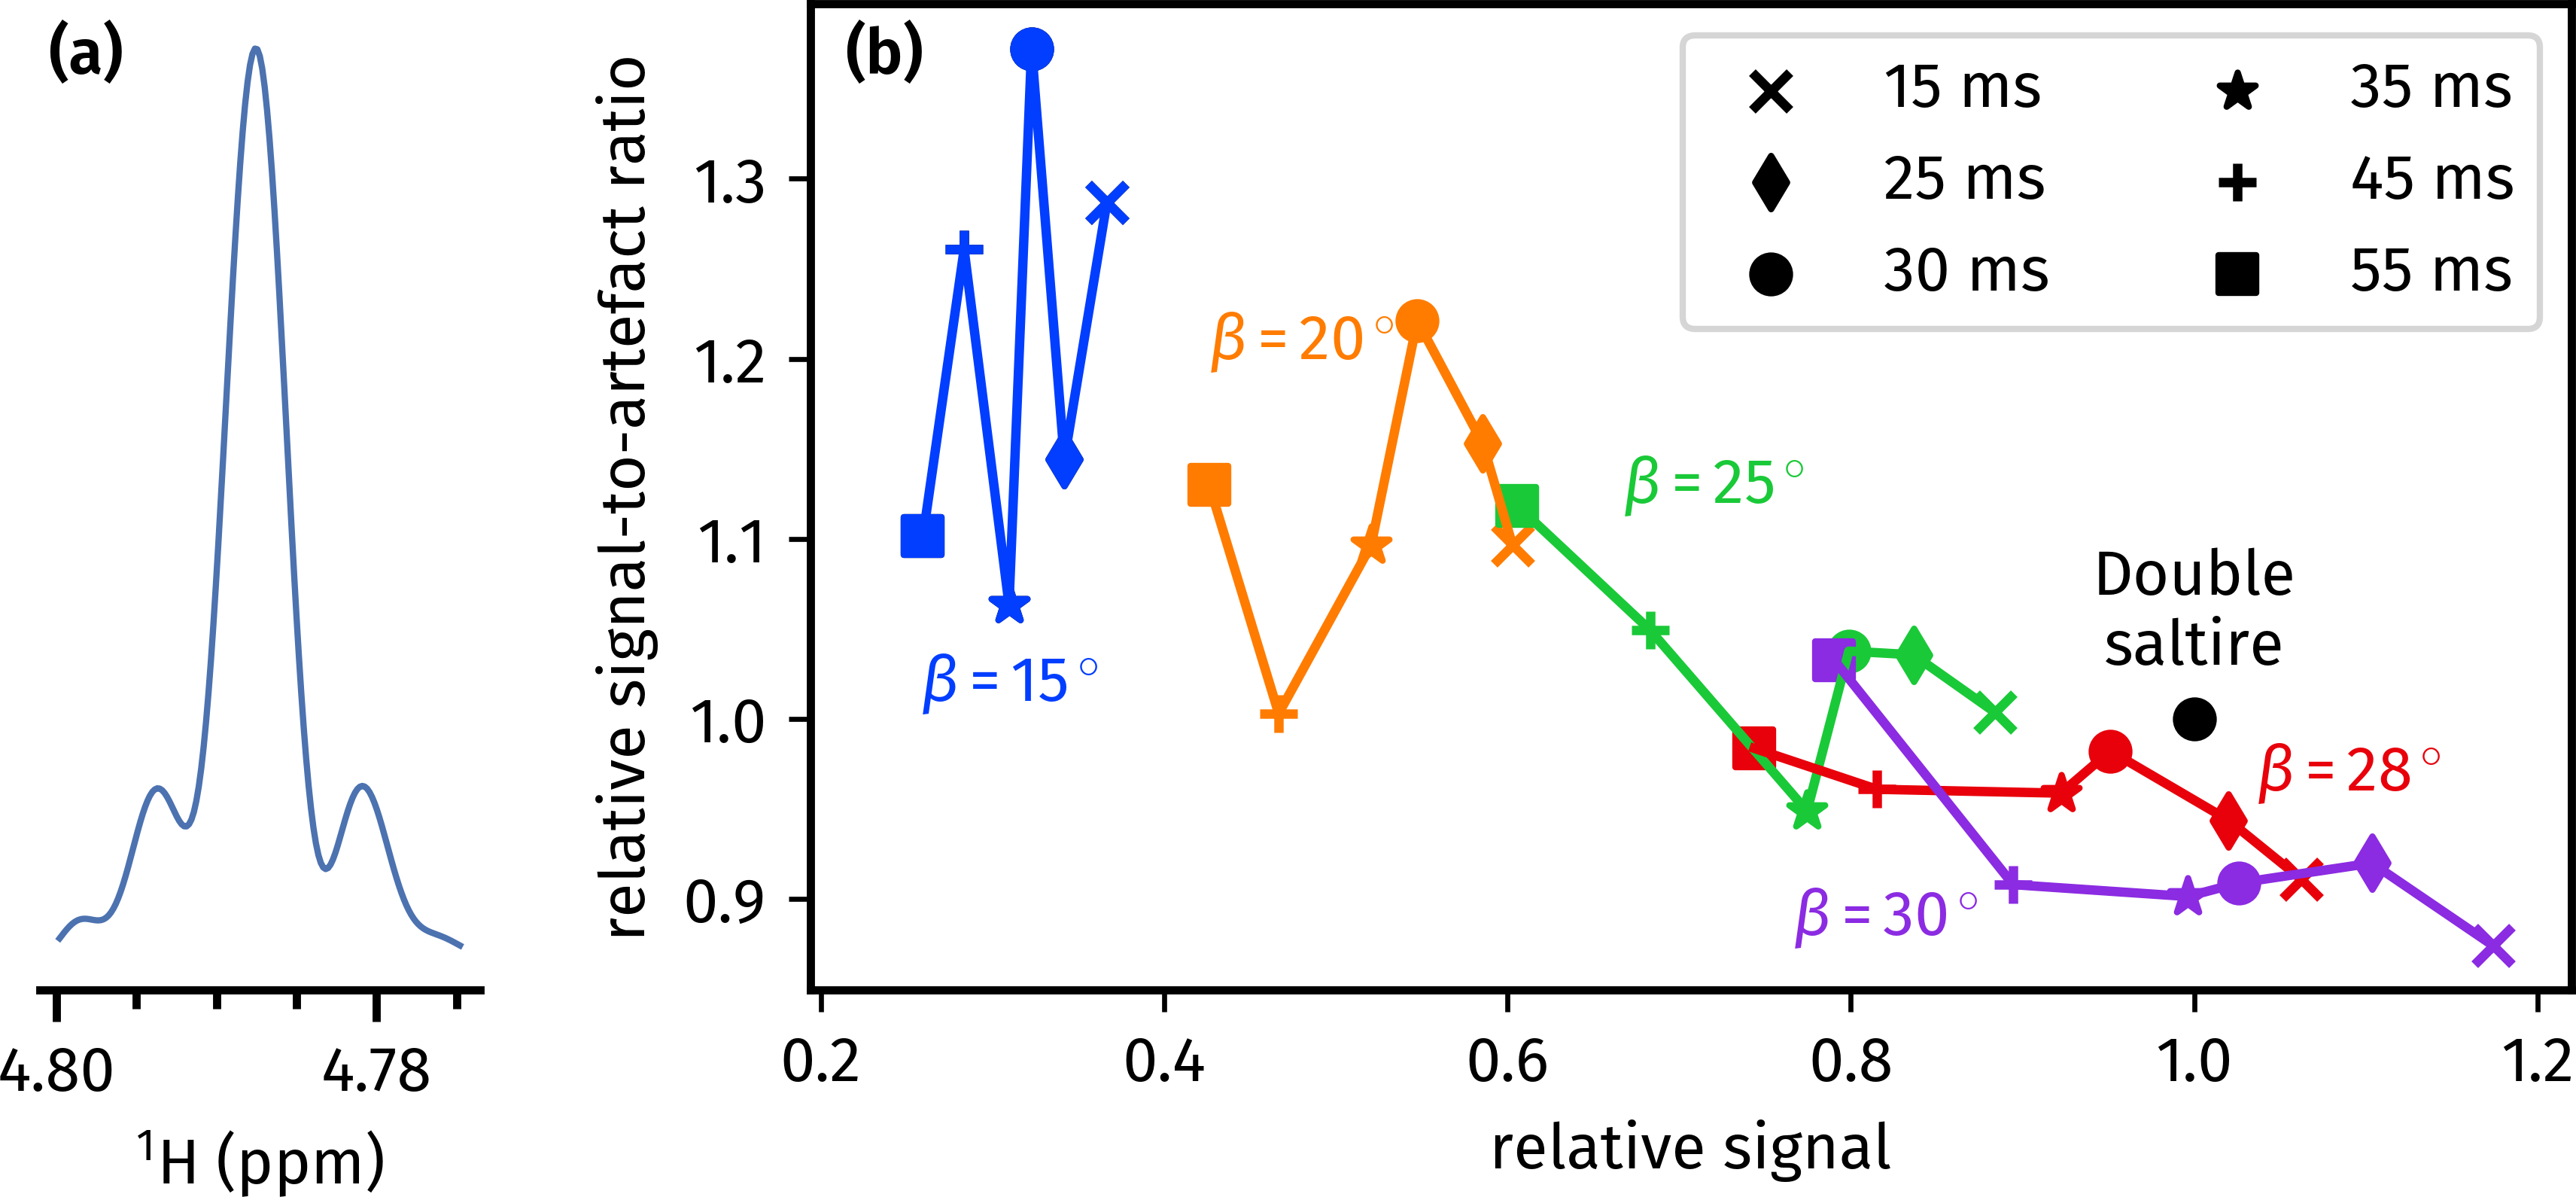
\includegraphics[]{pureshift/single_saltire.png}
    {\phantomsubcaption\label{fig:single_saltire_results_spec}}
    {\phantomsubcaption\label{fig:single_saltire_results_plot}}
    \caption[Single-saltire PSYCHE results]{
        \textbf{(\subref{fig:single_saltire_results_spec})} The peak in the (reference, double-saltire) pure shift spectrum of cyclosporin used for calculation of signal intensity and signal-to-artefact ratio.
        \textbf{(\subref{fig:single_saltire_results_plot})} Plot showing the signal intensity and signal-to-artefact ratio obtained in various single-saltire PSYCHE experiments, normalised against the double saltire experiment with $\beta = \ang{20}$ and $\taup = \SI{30}{\ms}$.
        Each line represents a series of single-saltire experiments acquired with the same value of $\beta$; $\taup$ generally decreases going left to right (i.e.\ a longer pulse means less signal). 
        \datacode{5C-190617}
    }
    \label{fig:single_saltire_results}
\end{figure}

The results thus obtained are shown in \cref{fig:single_saltire_results_plot}.
In this plot, both the sensitivities as well as the signal-to-artefact ratios are normalised with respect to the reference double-saltire experiment (black dot at $(1, 1)$, acquired using $\beta = \ang{20}$ and a total $\taup = \SI{30}{\ms}$, i.e.\ \SI{15}{\ms} per saltire).
An ideal PSE would fall in the top-right corner of this plot.
Clearly, as the flip angle increases, the sensitivity increases but at the cost of the purity: this is hardly unsurprising given that the double-saltire experiment has the same property.

While there is no standout candidate which is \textit{clearly} better than the double saltire (i.e.\ greater sensitivity as well as purity), the single-saltire pulse with $\beta = \ang{28}$ and $\taup = \SI{30}{\ms}$ comes close in performance to the double-saltire experiment.
(The use of $\beta = \ang{28}$ here is not coincidental: this flip angle for a single saltire was chosen to (approximately) match the sensitivity of the $\beta = \ang{20}$ double-saltire experiment.)
It is generally true that a shorter PSE yields to increased signal, and that usable results were obtained even with a simple \SI{15}{\ms} saltire.
However, a shorter PSE also leads to poorer spatiotemporal suppression of artefacts depends and thus poorer purity.

Both the single- and quadruple-saltire cases suffer from the classic dilemma of pure shift NMR: just as in the original PSYCHE, and in the Zangger--Sterk method before it, there is a compromise between sensitivity and purity, and one can only be increased at the cost of the other.
Arguably, then, there is not much value in changing the number of saltire pulses as simply varying the \textit{flip angle} of the basic double-saltire already gives the experimentalist a way to balance these competing objectives.
